\documentclass{article}
\usepackage{tikz}
\usetikzlibrary{graphs}
\usetikzlibrary{arrows.meta}

%\tracingall

\pgfkeys{
  /pgf/arrow keys/.cd,
  glyph text/.code={%
    \pgfarrowsaddtooptions{%
      \def\cdo@glyph{#1}%
    }%
  },
  glyph command/.code={%
    \pgfarrowsaddtooptions{%
      \def\cdo@glyph{\csname #1\endcsname}%
    }%
  }
}

\pgfdeclarearrow{
  name=BigGlyph,
  cache=false,
  bending mode=none,
  drawing code={
    \pgfpathrectangle{\pgfpoint{-1.5ex}{-1ex}}{\pgfpoint{+2ex}{+2.5ex}}
    \pgfusepathqclip
    \pgftransformxshift{+0.1ex}
    \pgftransformyshift{-0.8ex}
    \pgftext[right,base]{$\cdo@glyph$}
  }
}

\pgfdeclarearrow{
  name=SmallGlyph,
  cache=false,
  bending mode=none,
  parameters={},
  drawing code={
    \pgfpathrectangle{\pgfpoint{-1.5ex}{-1ex}}{\pgfpoint{+2ex}{+2.5ex}}
    \pgfusepathqclip
    \pgftransformxshift{+0.1ex}
    \pgftransformyshift{-0.5ex}
    \pgftext[right,base]{$\cdo@glyph$}
  }
}

\pgfdeclarearrow{
  name=phi,
  means={SmallGlyph[glyph command=phi]}
}

\begin{document}
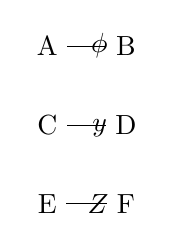
\begin{tikzpicture}
    \node (A){A};
    \node (B)[right of=A] {B};
    \node (C)[below of=A] {C};
    \node (D)[right of=C] {D};
    \node (E)[below of=C] {E};
    \node (F)[right of=E] {F};
    \draw [-phi] (A) to (B);
    \draw [-{SmallGlyph[glyph text=y]}] (C) to (D);
    \draw [-{BigGlyph[glyph text=Z]}] (E) to (F);
\end{tikzpicture}
\end{document}

